\begin{problem}
Find the best $L_1$ approximation to the function $f(x) = \sin(x) + \cos(x)$ in the interval $[\pi/3, 5\pi/3]$ from the space of polynomials of degree 2. Show that your result is indeed the unique best $L_1$ approximation to $f$.
\end{problem}

\begin{solution}
  By theorem (14.5 in Powell's book) if the approximation space is the
  space of polynomials of degree at most $n$, if $e^*$ has exactly
  $n+1$ zeros, then they are the extrema of the Chebyshev polynomial
  $T_{n+2}$. Therefore, by changing the interval from
  $[\pi/3, 5\pi/3]$ to $[-1,1]$ and finding the extrema, we get that
  the zeros of the error function are:
\begin{equation*}
  \xi_0 = \frac{\pi(3-\sqrt{2})}{3}, \quad \xi_1 = \pi, \quad \xi_2 = \frac{\pi(3+\sqrt{2})}{3}.
\end{equation*}
The polynomial we are trying to calculate has the form $ax^2+bx+c$, by
interpolating at the values calculated above $(p^*(\xi_i) = f(\xi_i))$
and solving the linear system, we should get the best approximation:
\begin{align*}
a\left(\frac{\pi(3-\sqrt{2})}{3}\right)^2+b\left(\frac{\pi(3-\sqrt{2})}{3}\right)+c &= \sin\left(\frac{\pi(3-\sqrt{2})}{3}\right) + \cos\left(\frac{\pi(3-\sqrt{2})}{3}\right) \\
a \pi + b\pi +c &=-1 \\
a\left(\frac{\pi(3+\sqrt{2})}{3}\right)^2 +b\left(\frac{\pi(3+\sqrt{2})}{3}\right) + c &= \sin\left(\frac{\pi(3+\sqrt{2})}{3}\right) + \cos\left(\frac{\pi(3+\sqrt{2})}{3}\right)
\end{align*}
This gives us the values $a=0.4150, b = -3.2803, c = 5.2091$, thus the
best approximation polynomial is:
\begin{equation*}
p^*(x)=0.4150x^2 -3.2803x+5.2091
\end{equation*}

To verify that this approximation is a best approximation we need to
be convinced that the error function only has 3 zeros. This is hard to
do analytically so the plot of the error function in figure
\ref{fig:task_3:error} will have to do. Fortunately the plot reveal
that there is exactly 3 zeros which fulfills the demands of theorem
14.5 and thus we can conclude that $p^*$ is a best approximation. 

\begin{figure}[!ht]
  \centering
  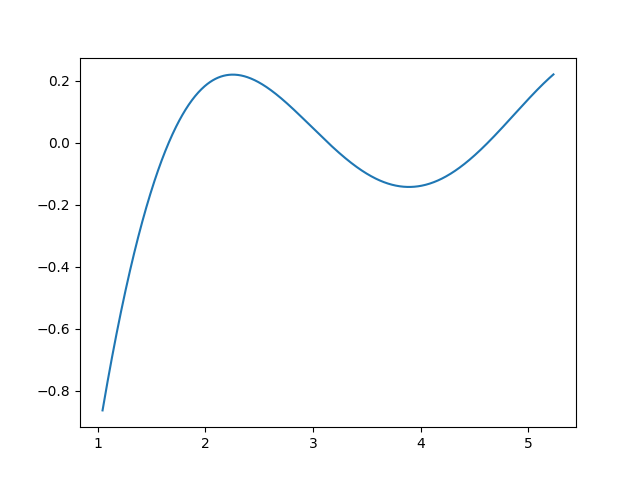
\includegraphics[scale = 0.5]{error.png}
  \caption{Plot of $f - p^*$. Note that there is exactly 3 zeros!.}
  \label{fig:task_3:error}
\end{figure}

As for uniqueness, we are approximating from the space of polynomials
of degree at most two, which is a Haar space, therefore by theorem
(14.3 in Powell's book) our best approximation is unique.
% By the characterization theorem, as the set
% $\mathcal{Z} = \{\xi_0, \xi_1, \xi_2 \}$ is composed of only discrete
% points, we have to show that:
% \begin{equation*}
% \int_{\pi/3}^{5\pi/3} s^*(x)p(x) \, \text{dx} = 0 \quad \forall p \in \mathcal{P}_2
% \end{equation*}
% where $s^*$ is defined as
% \begin{align*}
% s^*(x)=
% \begin{cases}
% (\phi_2, 1) = 0 \\
% (\phi_2, x) = 0
% \end{cases}
% \end{align*}
% It suffices to prove it for the monomial basis:
% \begin{align*}
% proof
% \end{align*}
\end{solution}


%%% Local Variables:
%%% mode: latex
%%% TeX-master: "report"
%%% End:
